\chapter{Introduction to Wireless Communication Systems}
We begin this report by providing an introduction to wireless communication systems in general and how the growth of wireless communication has lead to a new information revolution. We look at the motivation behind choosing this topic for our project and the objectives we wish to complete in our chosen field of study. A survey of the literature in this field is provided for the benefit of the reader, so that he/she may be acquainted with the current happenings in the field of mobile communication. Following this, a glimpse into the design methodology is given and the constraints set on the project which define the scope within which our research is applicable.    

\section[Introduction]{\textbf{Introduction}}
Guglielmo Marconi invented the wireless radio system in 1895, and since then wireless communication has grown to become ubiquitous. As of 2018, there are 5.1 billion unique mobile phone users with this number expected to touch 5.8 billion between 2018-2025. \parencite{George2017}.
In all this time, the basic components of a wireless communication systems have remained the same as shown in Figure. 
\ref{fig:wireless block diagram}
\begin{figure}[htb]
\centering
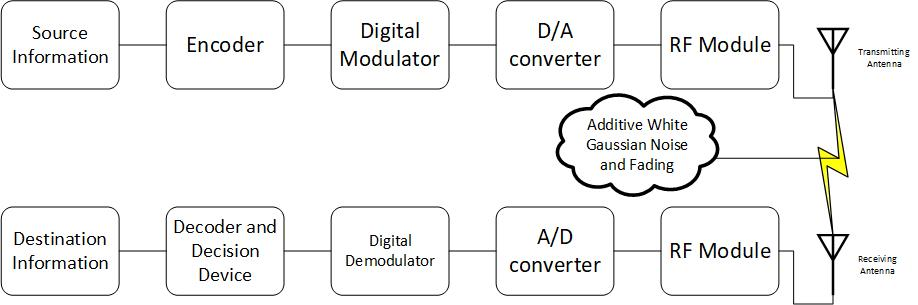
\includegraphics[scale=0.8]{Chapter 1/Figures/Wireless Communication System Block Diagram}
\caption{Wireless Digital Communication System}
\label{fig:wireless block diagram}
\end{figure}
 
In further chapters we discuss the various components of this system and the different techniques we used in implementing them in \gls{matlab}. In this report we are only concerned with the digital aspects of the system and we do not pay much attention to the antenna parameters which can have a significant role to play in wireless systems. 


\section[Motivation]{\textbf{Motivation}}
There is an exponential increase in the number of new mobile users being added every year. Also, there are a host of services available for mobile users which demand high data rates. Video Teleconferencing, Real Time Video Streaming and other such services are some examples. These services coupled with the large number of people subscribing to such services means that there is a requirement for high capacity and high data rate systems.\\

At present the state of the art \acrshort{mimo} system is only being used in \gls{spatial diversity} mode which limits the capacity of the mobile system. Hence, it becomes attractive for telecom service providers to use the existing \acrshort{mimo} systems in \gls{spatial multiplexing} mode as well so that capacity is increased and at the same time maximum possible data rates are achieved for existing channel \acrshort{snr} conditions.  

\section[Problem statement]{\textbf{Problem statement}}
The problem statement which we try to address in this report is the implementation of suitable \acrshort{mimo} models for urban cellular links that can help to increase the capacity of the system.

\section[Objectives]{\textbf{Objectives}}
The objectives of the project are
\begin{enumerate}
\item To develop an effective channel model for $2 \times 2$ \acrshort{mimo} links
\item To develop an efficient transmitter and receiver supporting \acrshort{mcm} and \acrshort{mimo} processing.
\end{enumerate}

\section{Literature Review}

\subsection{Multicarrier Systems}
The backbone of modern day \acrshort{4g} and \acrshort{5g} systems is the paradigm shift from single-channel systems to multi-carrier systems. We build upon the work of \parencite{Weinstein and Ebert} where they offer a low cost and easy to implement solution with the help of an \acrshort{ifft} and \acrshort{fft} blocks which allows the system designer to use a single modulator rather than a block of modulators for each subchannel. This coupled with multiplexing capabilities of \acrshort{ofdm} as discussed by \parencite{Wu and Zou} form the foundation upon which our project is based.
 
\subsection{Modulation and Precoding Schemes}

\subsubsection{Modulation Schemes}
Coming to digital modulation schemes available at our disposal, we have decided to use \acrshort{qam} as it is best suited for our purposes. However, to achieve effective higher order \acrshort{qam} constellations we follow in the work of \parencite{Bellili} to use a recursive algorithm that effectively maps symbols to higher order constellations in a computationally inexpensive manner. This method starts with the basic 4\acrshort{qam} and 8\acrshort{qam} constellations and dynamically creates higher order constellations without the need to save the points in memory.

\subsubsection{Precoding Schemes}
In certain cases, like $2 \times 1$ \acrshort{miso} systems where we choose to go for \gls{spatial diversity} scheme, we include some precoding measures as suggested by \parencite{Alamouti} so that we can ease the burden on our system and improve overall system performance.

\subsection{Channel Modeling}
In terms of modeling the real world channel, we must consider various random processes to accurately define the channel. However, for the sake of simplicity we find it easier to model multipath systems as previously shown by \parencite{Hanlen and Fu} where we place more importance on \gls{rayleigh fading} and ignore other effects like those of shadowing. Although, \gls{rayleigh fading} is a statistically simple model, it serves us well in showing the effects of fading on data signals while at the same time keeping complexity low. Channel estimation becomes an integral part of wireless systems as it directly correlates with the accuracy of our receiver and thereby our system performance.\\
Along with modeling fading, we also take into consideration the aspects of noise that the channel adds to our data signal. Similarly as before, we have chosen \acrshort{awgn} type of noise to represent an accurate but simplistic model. In our survey we have noticed that most research scholars stick to a similar approach and we have decided to follow in their footsteps.


\subsection{Transceiver Architecture and Channel Loading Methods}
\subsubsection{Transceiver Architecture}
In the design of our transmitter and receiver systems, we have relied upon standards set by the \acrshort{itu} as per their technical document \parencite{ITU2009}. We build upon the \gls{pilot signal} generation scheme provided here and suggest an alternative scheme with two $M \times N$ \acrshort{lfsr} banks to increase the dynamic range of the \acrshort{prbs} generator by observing the results of \parencite{Peinado}. We also follow the same \parencite{ITU} standard in designing our transmitter and receiver systems to remain compliant with existing market service providers. The improvisation for the receiver comes in the form of \acrlong{svd} method as described by \parencite{Klema and Laub}. It is our claim that this method enhances the system performance while reducing complexity making it commercially viable and attractive. 

\subsubsection{Channel Loading Methods}
Effective channel loading not only helps users with improving data rates but is also required for service providers to improve spectral efficiency. In our study of the existing literature we found that the method followed by \parencite{Chow and Bingham} to be effective but unsuitable as it is rate adaptive in nature. Therefore, we drew inspiration from this tone loading algorithm to define our own fine gains algorithm to achieve an effective bit loading scheme. This loading scheme uses directly builds on the seminal work of \parencite{Shannon} and satisfies our requirements well while also being highly optimal.


\section{Brief Methodology of the project}
We first begin by developing a \acrlong{prbs} generator, abbreviated as \acrshort{prbs} generator to generate \glspl{pilot signal} for the purposes of channel estimation. Then, load these bits onto the channel with the help of an adaptive tone loading algorithm. We then develop a \acrshort{qam} constellation mapper and \acrshort{qam}. modulator to map the bits to \acrshort{qam} symbols. Along with this, suitable encoders like Alamouti encoders are added to form the transmitter end of the system.\\
By transmitting the \glspl{pilot signal} we determine the channel characteristics and model it to our satisfaction and use this information at the receiver to decode the bits correctly.\\
Similar to the transmitter, the receiver contains Alamouti decoder, and \acrshort{qam} demodulator to obtain the transmitted signal. Finally we measure the system performance by looking at the \acrlong{ber}, abbreviated as \acrshort{ber} and measure the effectiveness of our system.

\section{Assumptions made / Constraints of the project}
Some of the constraints we have set for our project are as follows.
\begin{enumerate}
\item We only introduce \gls{rayleigh fading} in our channel and focus on \acrshort{los} paths. We do not focus on other delayed paths in the channel.
\item All the channel parameters including \acrshort{snr} tables and channel coefficients have been provided to us by our guide.
\item The distance of separation between the transmitter and receiver is taken to be $1Km$.
\item The transmitter is assumed to be operating on a power budget of $1mW$.
\item The antenna design parameters are not focused upon but are approximated to the values of \acrshort{gr} and \acrshort{gt}.
\item The system is taken to be operating in the frequency range of $1 MHz$.
\item We are limiting the number of bits transmitted to around $10^7$ to measure our \acrshort{ber}.
\end{enumerate}

\section{Organization of the report}

This report is organized as follows. 
\begin{itemize}
\item Chapter 2 discusses the fundamentals of \acrshort{mcm} and \acrshort{mimo} systems. We discuss the key technologies in \acrshort{mcm} and \acrshort{mimo} that enable it to be an effective solution for modern cellular systems. Along with this we also discuss some of the challenges faced in their implementation.
\item Chapter 3 informs the reader about the steps we have taken to design our communication system delving into the details of the design parameters and algorithms used. 
\item Chapter 4 shows the results we have obtained by performing simulations of our system on \gls{matlab}. We show the comparison of performance  between existing systems and our system and highlight the effectiveness of our system.
\item Chapter 5 is the final chapter where we conclude our report and mention the scope for future research and list some additional features that can be added to our system to improve it. 
\end{itemize}

